\documentclass{article}
\usepackage{graphicx} % Required for inserting images
\usepackage{booktabs} % For better table formatting
\usepackage{array}    % For more flexible table features
\usepackage{placeins} % To control figure placement

\title{Analysis of Single Mutants}
\author{Your Name} % Replace with your name
\date{}

\begin{document}

\maketitle

\section*{Introduction}
To guide the selection of mutations for directed evolution, a multiple sequence alignment was performed between the human and mouse wild-type protein. This MSA revealed 47 positions that differed between the human and mouse sequences, suggesting potential sites for mutagenesis. In order to prioritize residues for mutagenesis, the distances from the alpha carbon of Cys/Sec49 (active site residue) and the rest of the 46 positions were calculated. Residues were then grouped into distance criteria of <10 Å, 10-15 Å, 15-20 Å, 20-25 Å, 25-30 Å, and 30-35 Å. This distance-based approach allowed us to select residues within different proximity ranges to Cys/Sec49. Grouping residues into distance bins provides a systematic and stochastic way to explore the impact of mutations at varying distances from the target residue (Cys/Sec49). 

To investigate the individual contributions of each residue to the structural and functional differences between the human and mouse proteins, single mutants were generated systematically. Each mutation corresponds to substituting a residue in the mouse protein with its human counterpart, or vice versa, as outlined in the mutation table of 47 residues. This process was conducted one residue at a time to isolate the effects of each mutation.

The mutations were applied by transferring each residue from the mouse sequence to the human sequence and vice versa, ensuring a controlled and systematic approach to mutagenesis. The active site residue, Cys/Sec49, remained a fixed reference point, with all mutations being calculated relative to it. For example, residues such as position 3 (N to K) and position 4 (R to S) involved changes in side-chain polarity or charge, while others, such as position 48 (Y to F), focused on aromatic substitutions. These single-residue changes allow for direct comparisons of the energetic and structural effects of each mutation, enabling us to study how these variations influence activation barriers and overall protein function.

By analyzing the 47 single mutants, we aim to systematically explore the structural transitions and activation energy changes associated with the human-to-mouse and mouse-to-human sequence transformations. This stepwise approach ensures that the contributions of individual residues to protein evolution and function are thoroughly characterized.

\begin{figure}[h!]
    \centering
    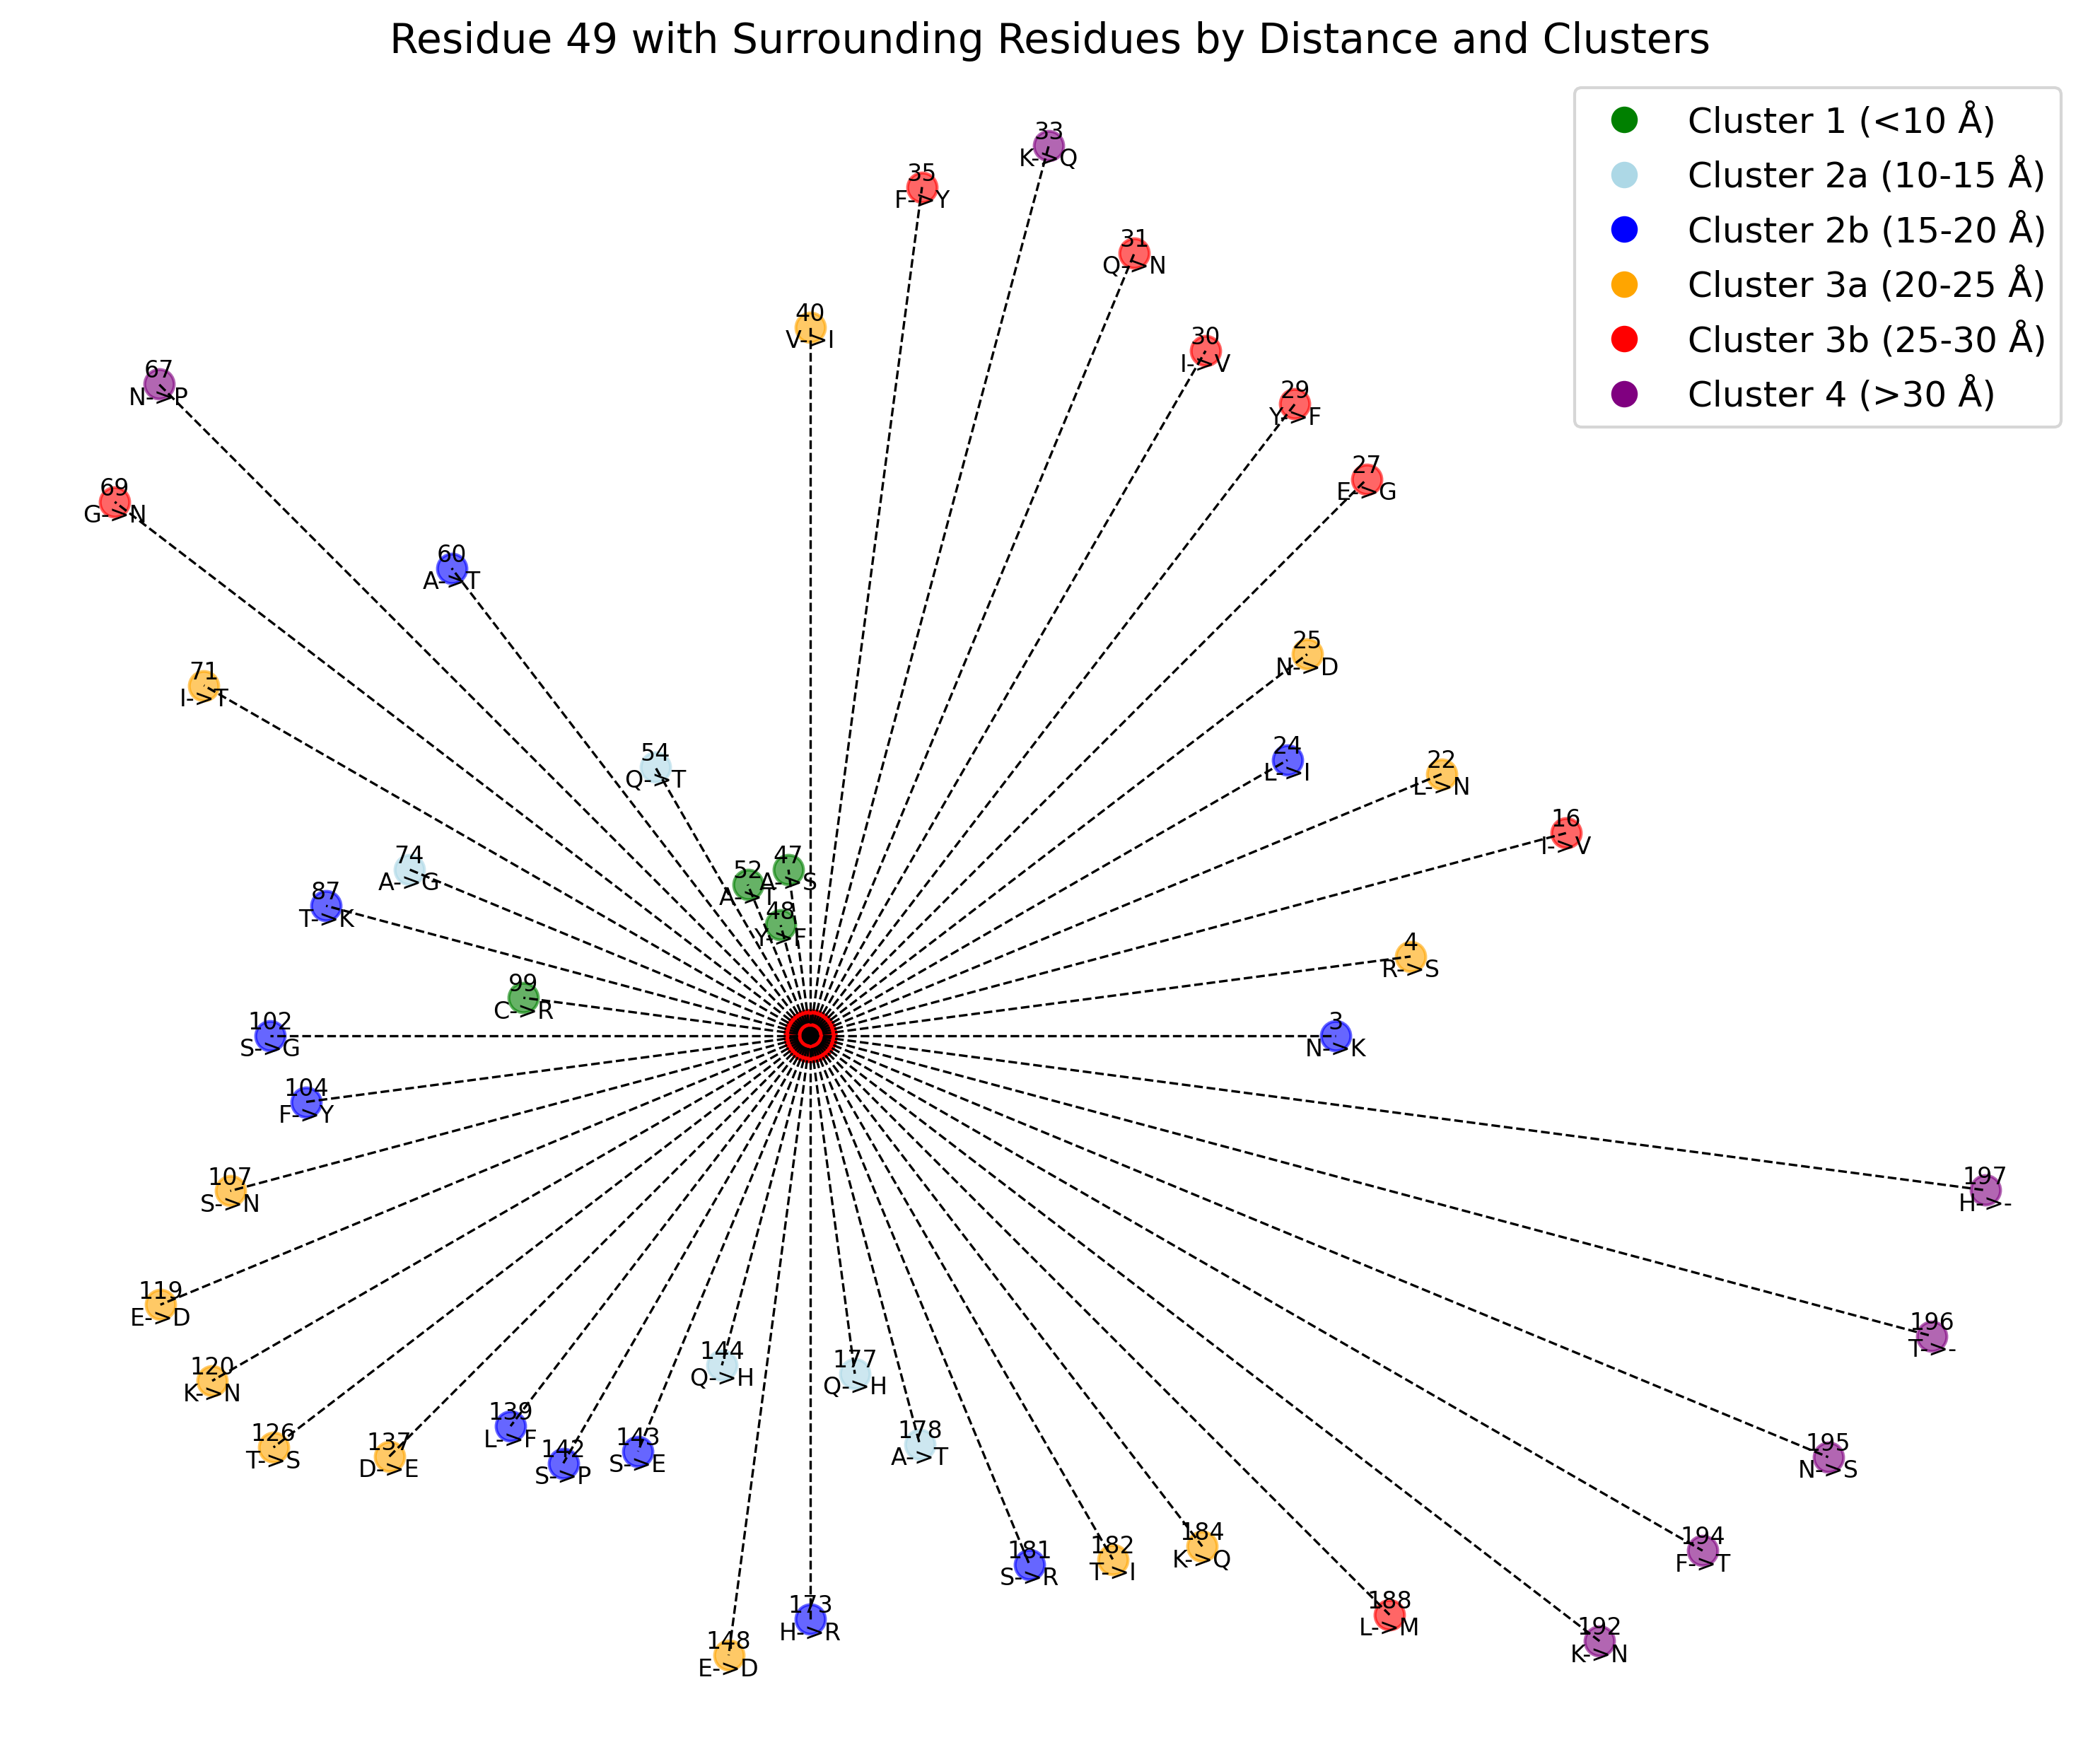
\includegraphics[width=0.8\linewidth]{/home/hp/nayanika/github/GPX6/figures/Residue_human_Distances.png} % Replace with your image file name
    \caption{Distance of residues from the active site for human mutants. The figure highlights proximity of each residue to Cys/Sec49.}
    \label{fig:human_distances}
\end{figure}

\begin{figure}[h!]
    \centering
    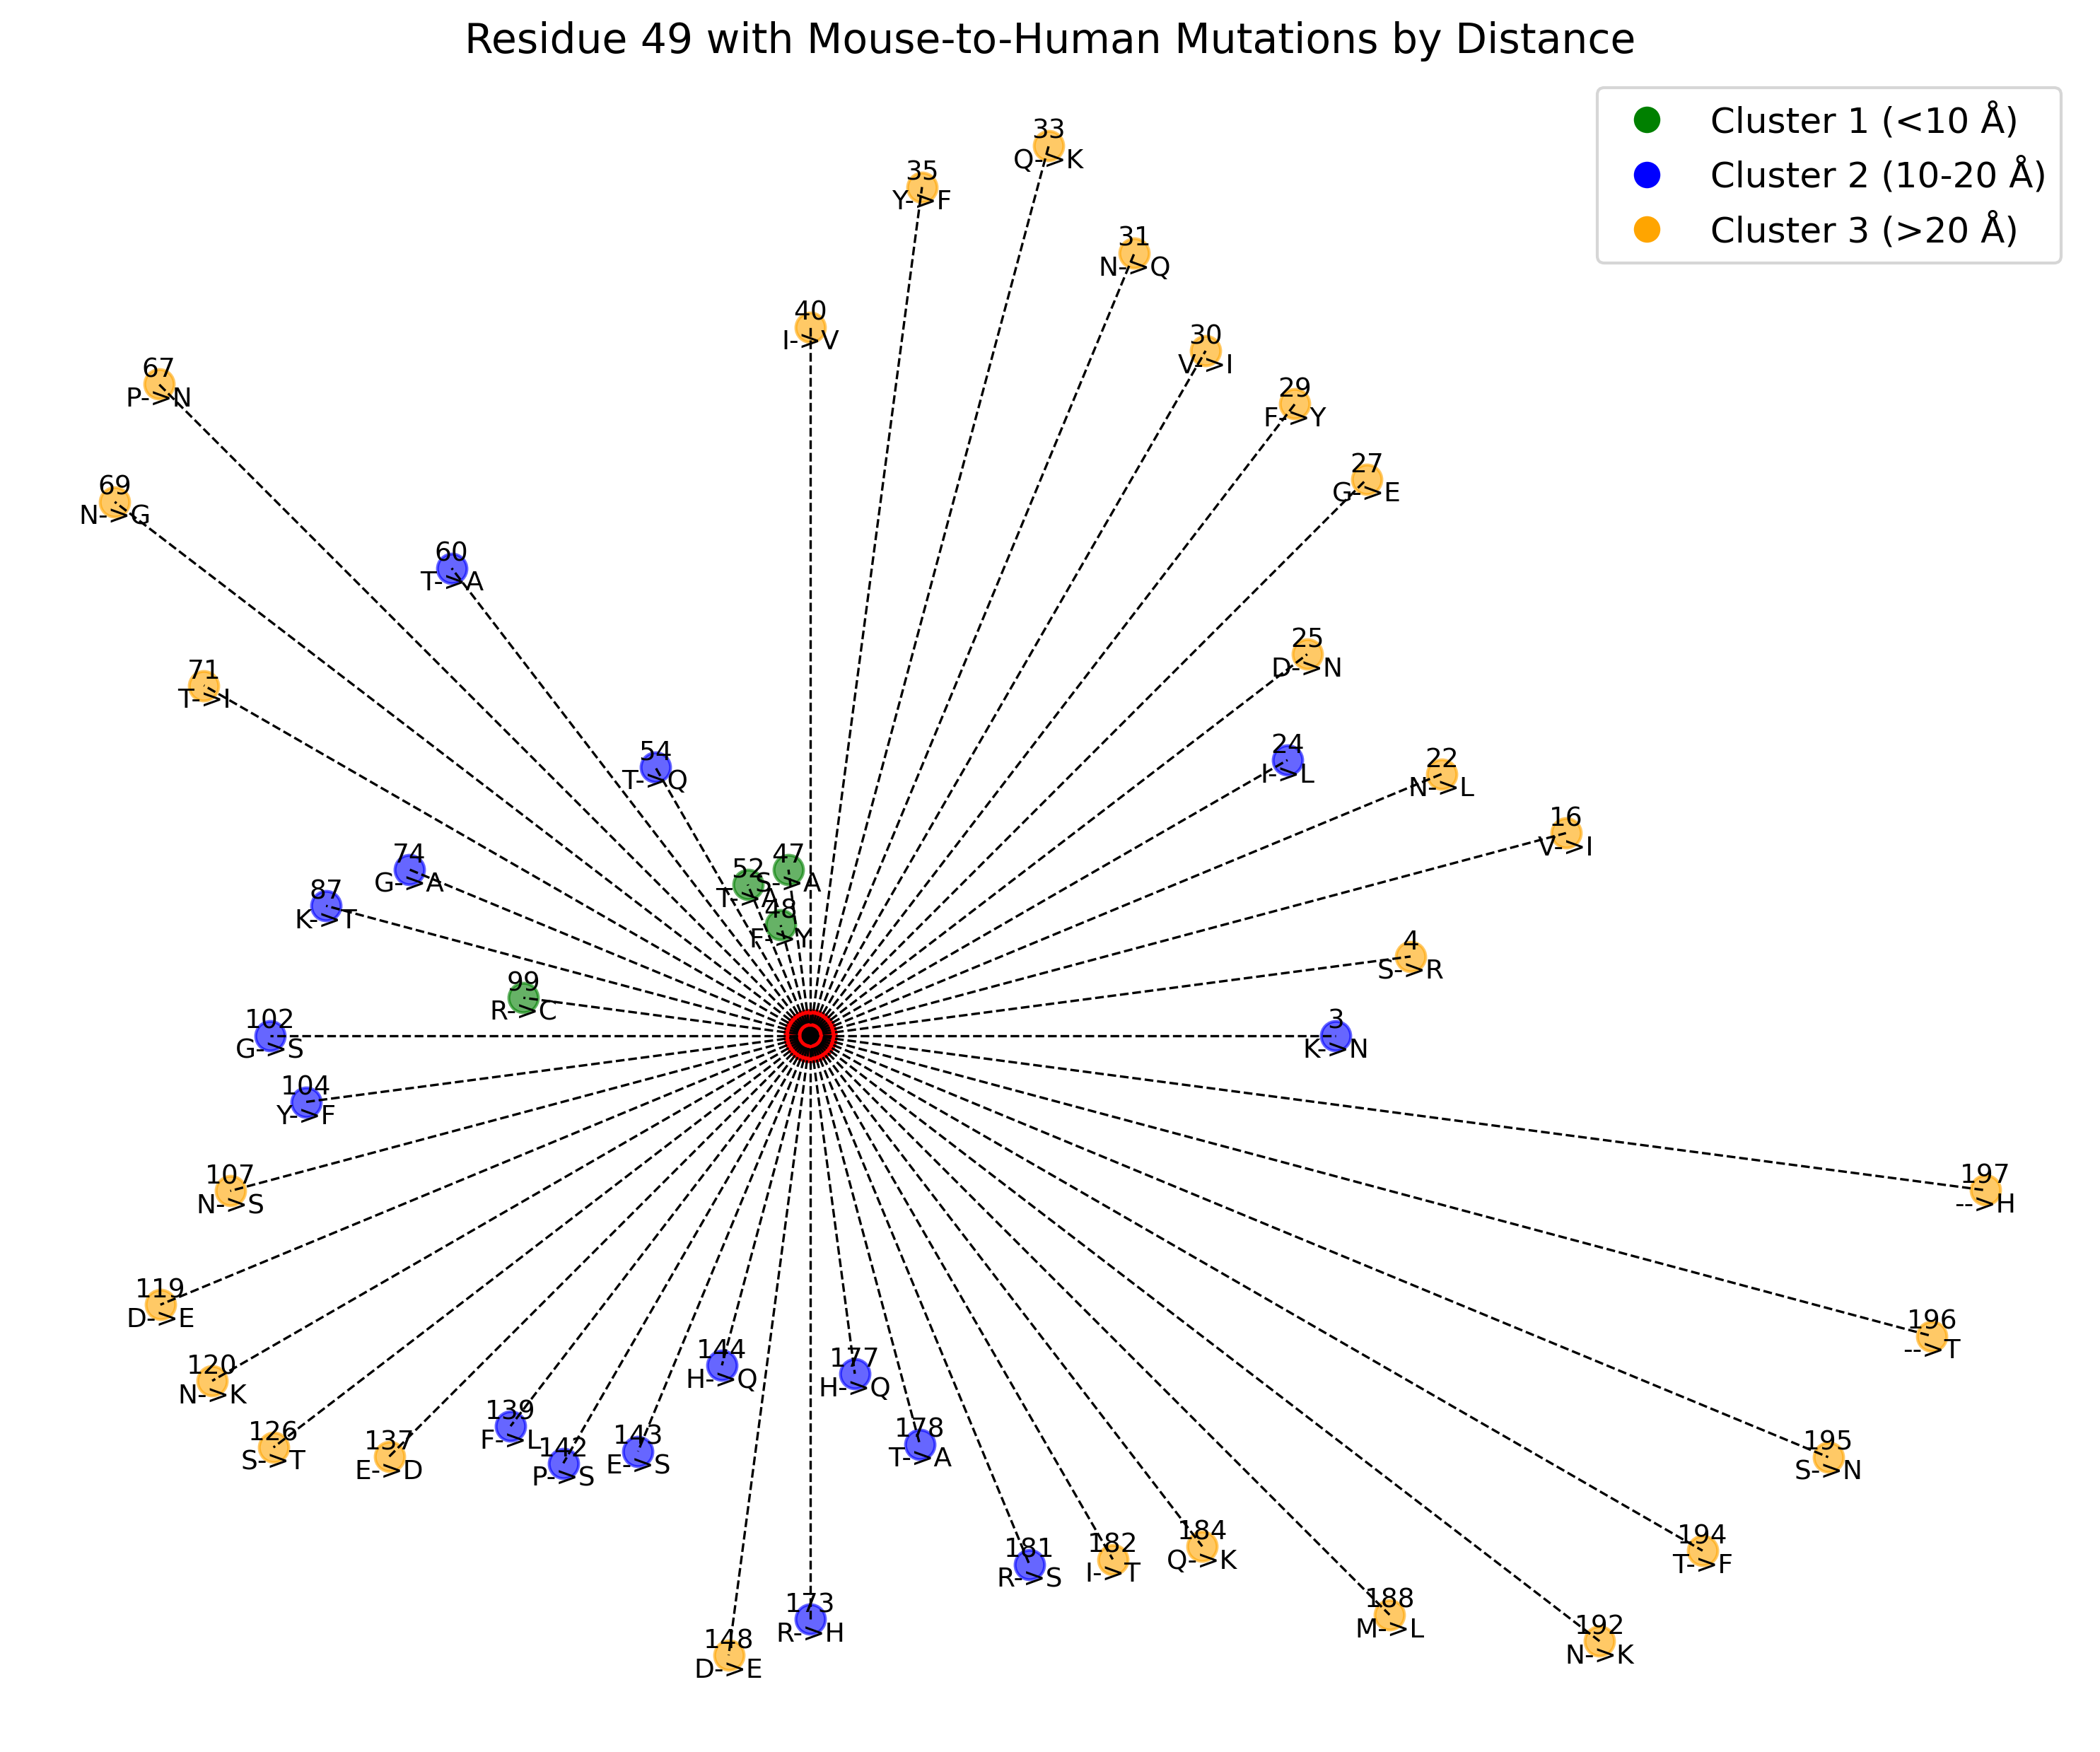
\includegraphics[width=0.8\linewidth]{/home/hp/nayanika/github/GPX6/figures/Residue_mouse_Distances.png} % Replace with your image file name
    \caption{Distance of residues from the active site for mouse mutants. The figure highlights proximity of each residue to Cys/Sec49.}
    \label{fig:mouse_distances}
\end{figure}

\subsection{Clustering the Variants}

The image below shows a 3D scatter plot of residues clustered based on their spatial proximity, hydrophobicity, and free energy values. The analysis begins by extracting residue data from a PDB file, where each residue’s position and amino acid identity are mapped. The residues are represented by their 3D coordinates, which are then used to compute pairwise distances. These distances are input into the KMeans clustering algorithm to group residues spatially, with the optimal number of clusters determined using the Elbow Method.

Residues are color-coded based on their **hydrophobicity** (a physicochemical property) to highlight how the hydrophobicity influences the clustering. The clustering provides insight into spatial relationships and physicochemical properties that might play a role in protein function.

\begin{figure}[h!]
    \centering
    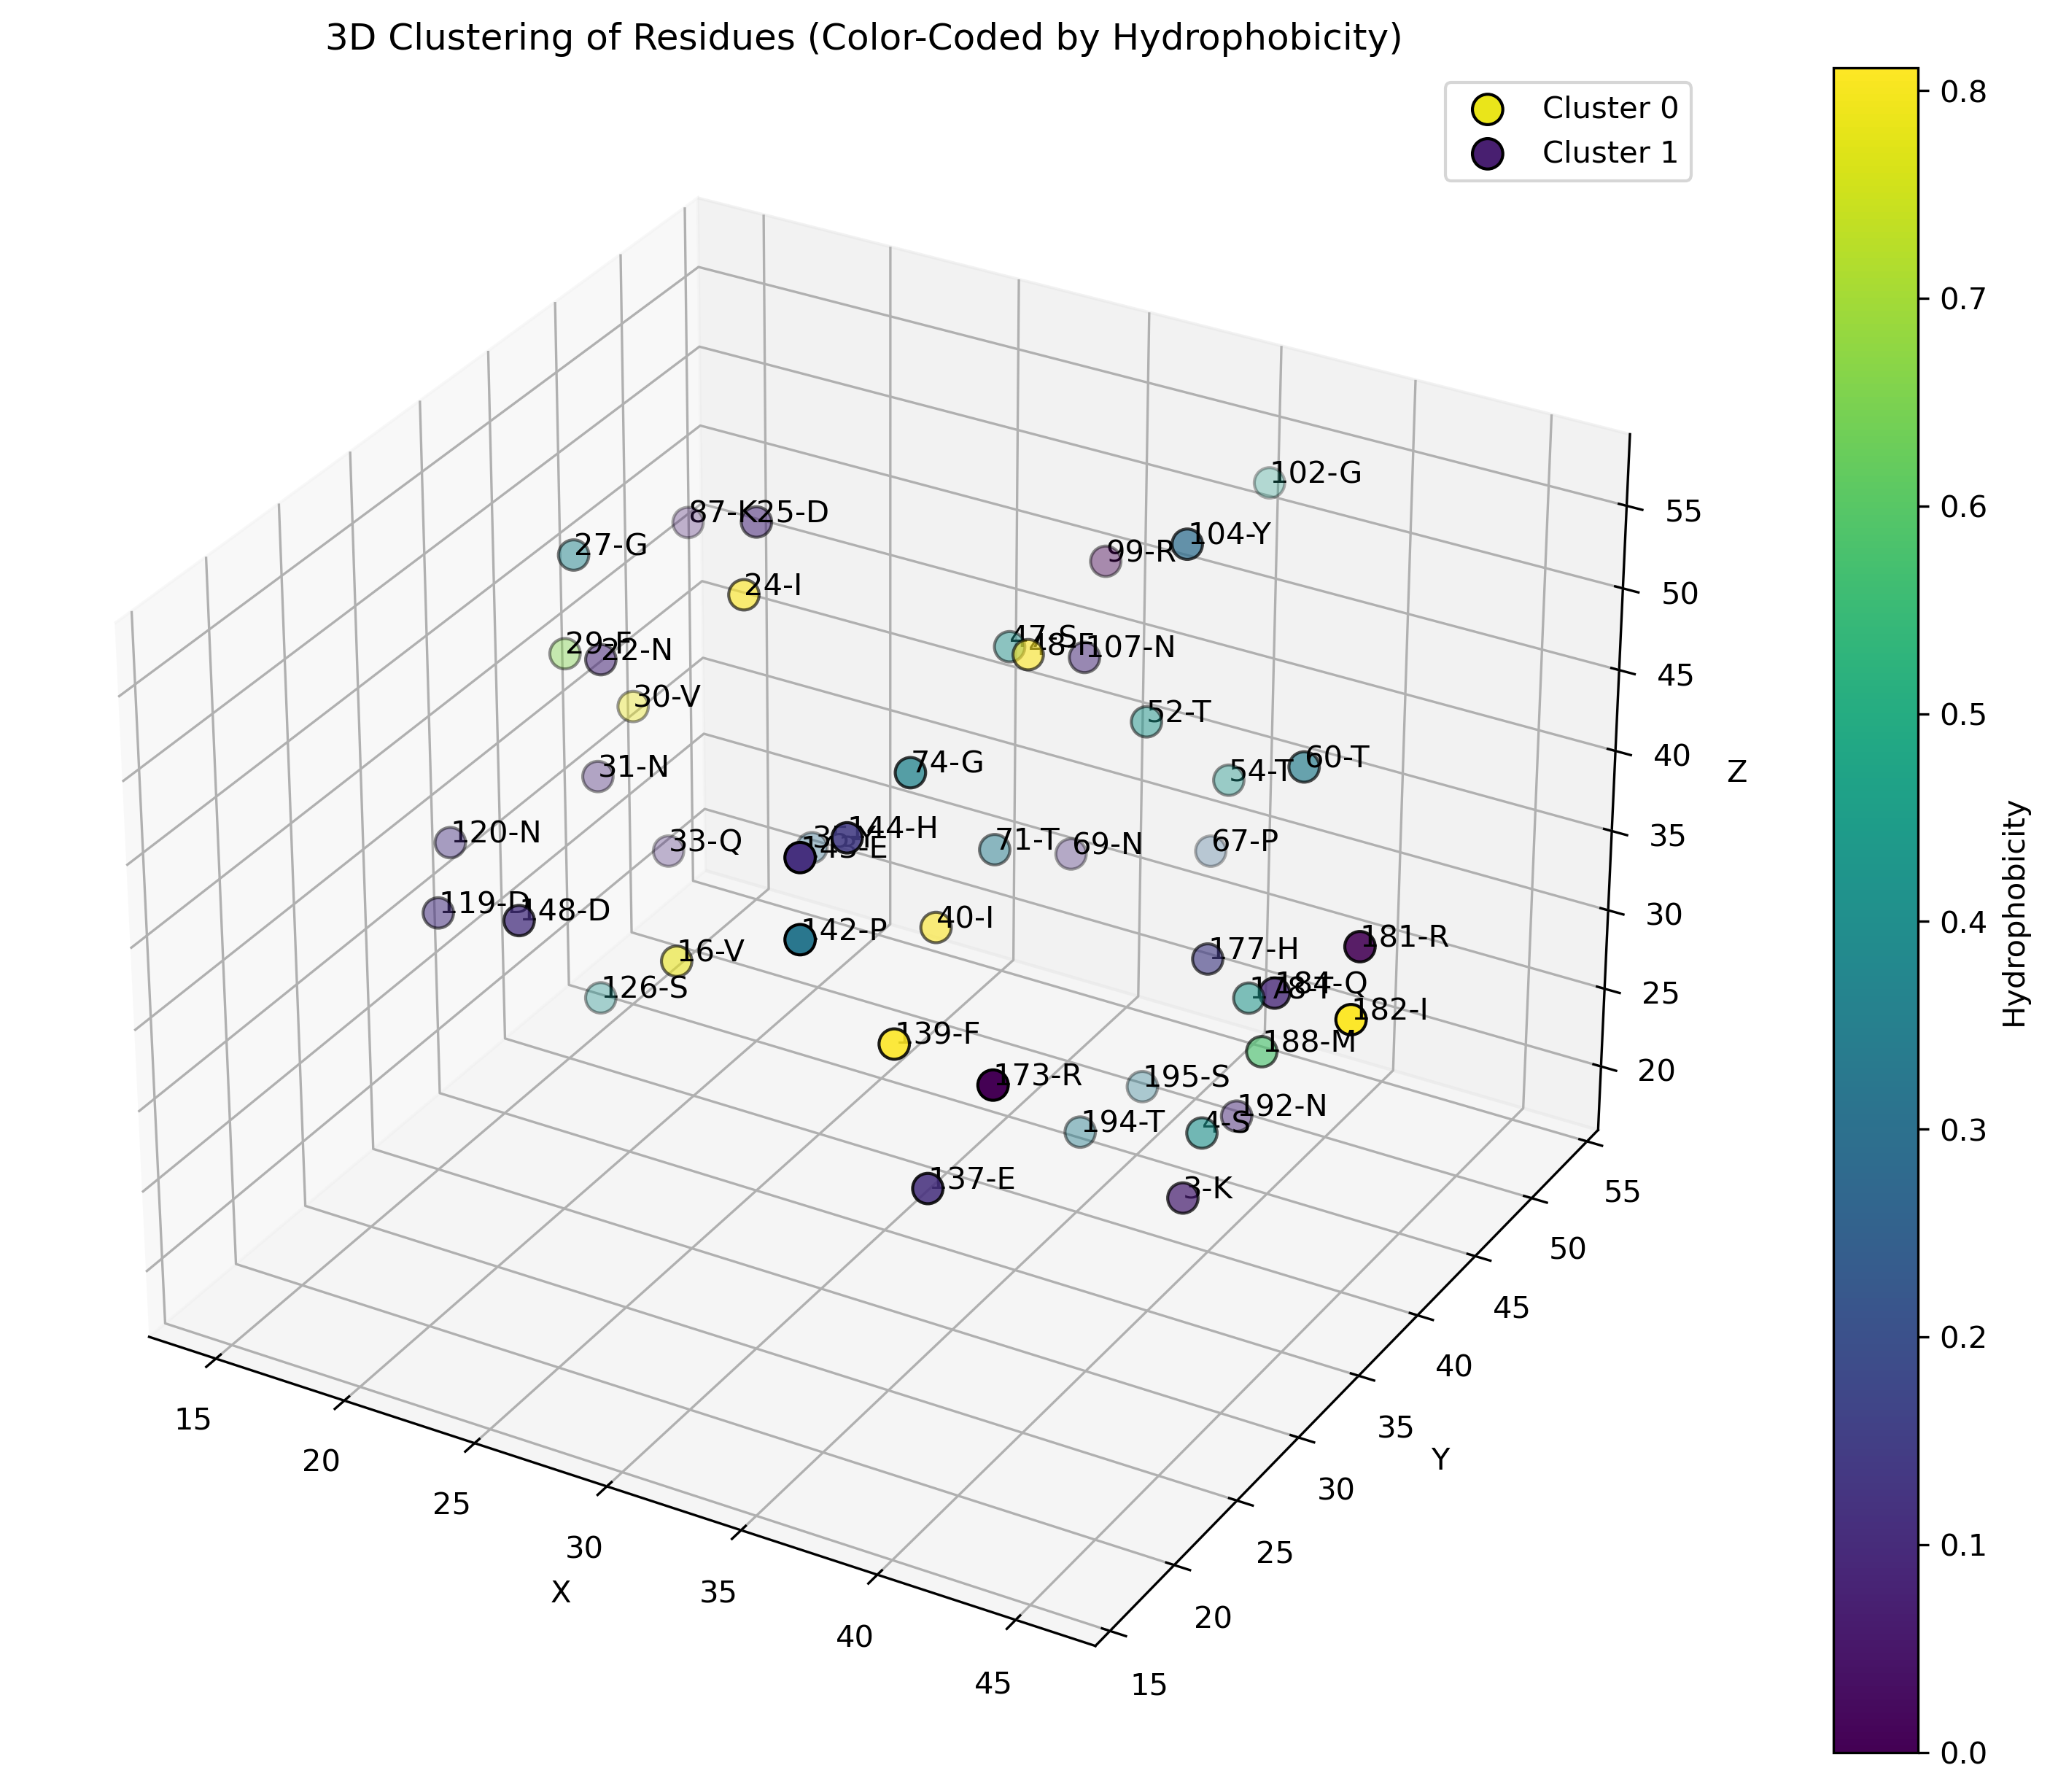
\includegraphics[width=0.8\linewidth]{/home/hp/nayanika/github/GPX6/figures/3d_clustering_residues.png} % Replace with your image file name
    \caption{3D clustering of residues based on spatial proximity, hydrophobicity, and free energy values. Each cluster represents residues grouped by their spatial location and physicochemical properties.}
    \label{fig:3d_clustering}
\end{figure}

\subsection{Visualizing the Clusters}

The following figure illustrates the clustering of mutants based on the distances from the active site and other relevant features. This visualization provides a clear representation of how mutations at different positions affect the protein’s structure and potential function.

\begin{figure}[h!]
    \centering
    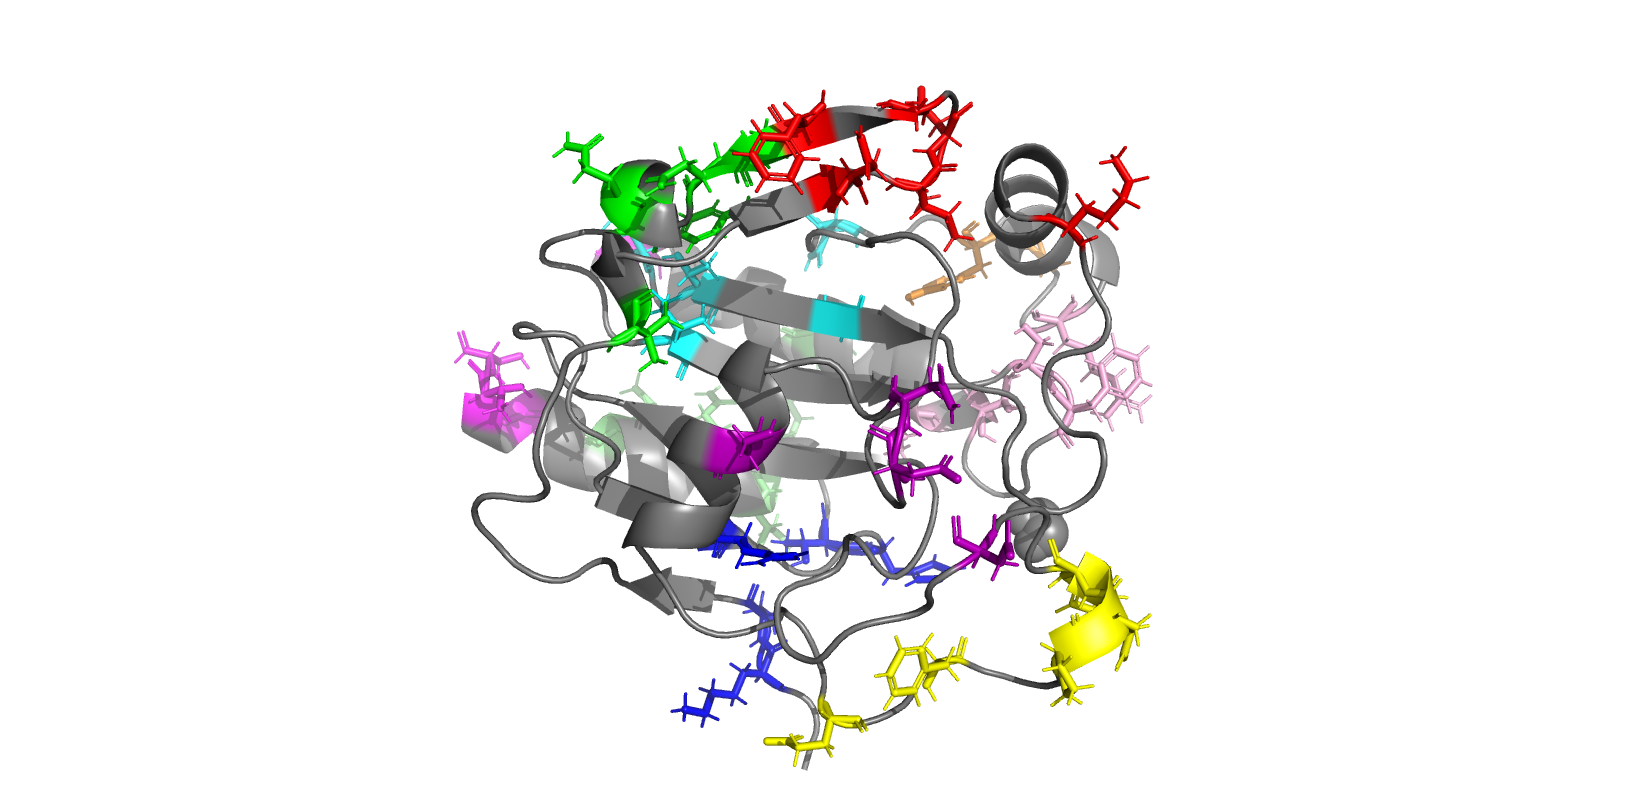
\includegraphics[width=0.8\linewidth]{/home/hp/nayanika/github/GPX6/figures/clustered_mutants.png} % Replace with your image file name
    \caption{Visualization of clustered mutants showing the proximity of residues to Cys/Sec49. The clusters reveal how residue variations may affect protein stability and function.}
    \label{fig:clustered_mutants}
\end{figure}

\end{document}
